\documentclass{article}

\usepackage[utf8]{inputenc}
\usepackage{fixltx2e}
\usepackage{graphicx} 
\usepackage[a4paper, total={6in, 8in}]{geometry}
\usepackage{enumitem}

\author{Marc Juvillà Garcia}
\title{Homework 1. Machine Learning (MIIS)}

\begin{document}
\maketitle

\begin{enumerate}[label=(\alph*)]
\item Generate a dataset of size 20. Plot the examples \{(x\textsubscript{n} , y\textsubscript{n})\} as well as the target function \textit{f} on a plane.
\begin{center}
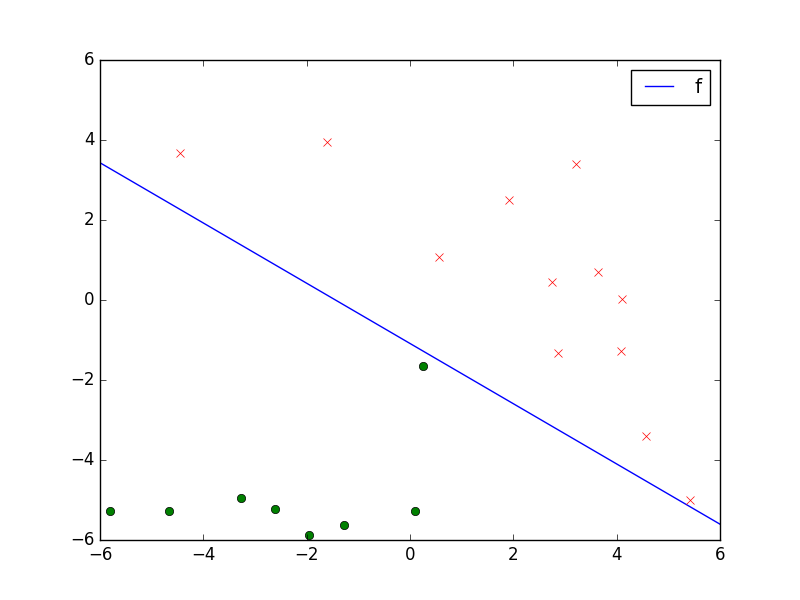
\includegraphics[scale=0.4]{images/1.png} 
\end{center}

\item Run the perceptron algorithm on the dataset. Report the number of updates that the algorithm takes before converging. Plot the examples \{(x\textsubscript{n} , y\textsubscript{n})\}, the target function \textit{f}, and the final hypothesis \textit{g} in the same figure.
\begin{center}
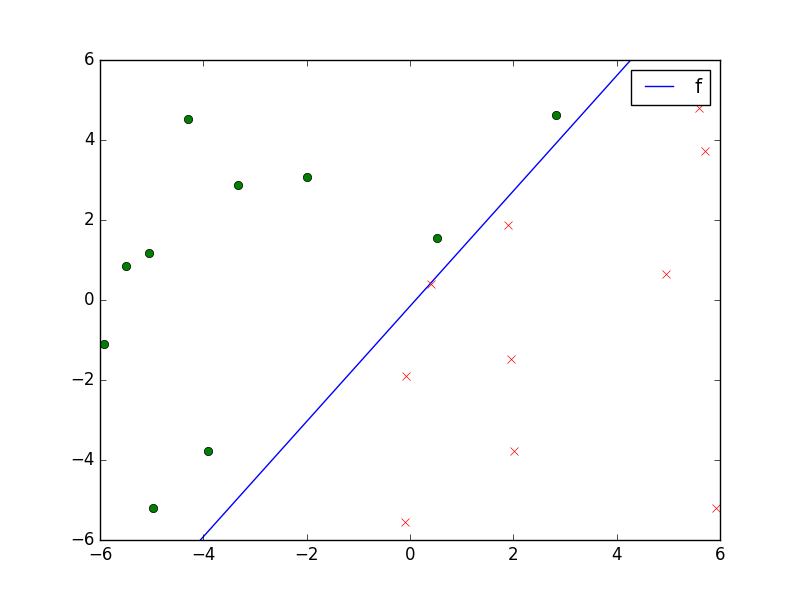
\includegraphics[scale=0.35]{images/2_a.png} 
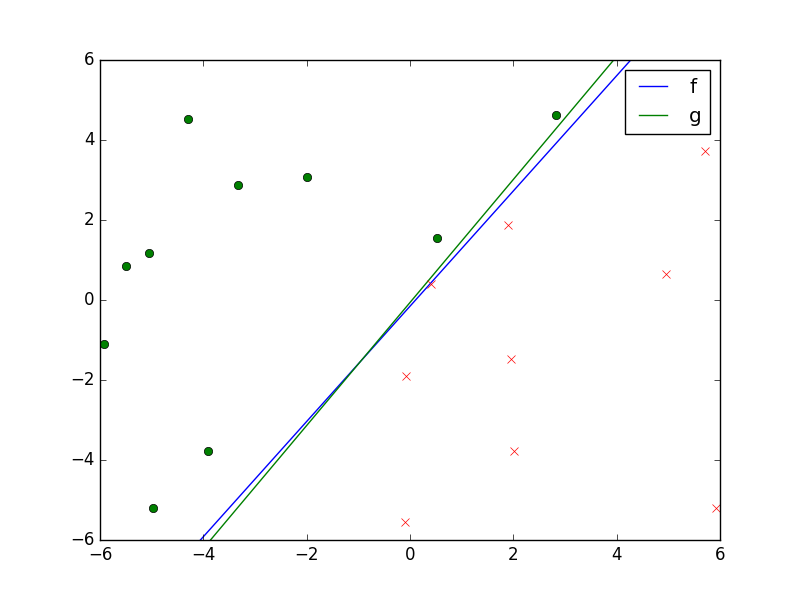
\includegraphics[scale=0.35]{images/2_b.png} 
\end{center}
For the model shown in the figures, it took 12 updates of the model (that is, correcting 12 mistakes) and 0.292 ms before converging. 

\item Repeat everything in b) with another randomly generated dataset of size 20, and compare the result to b).
\begin{center}
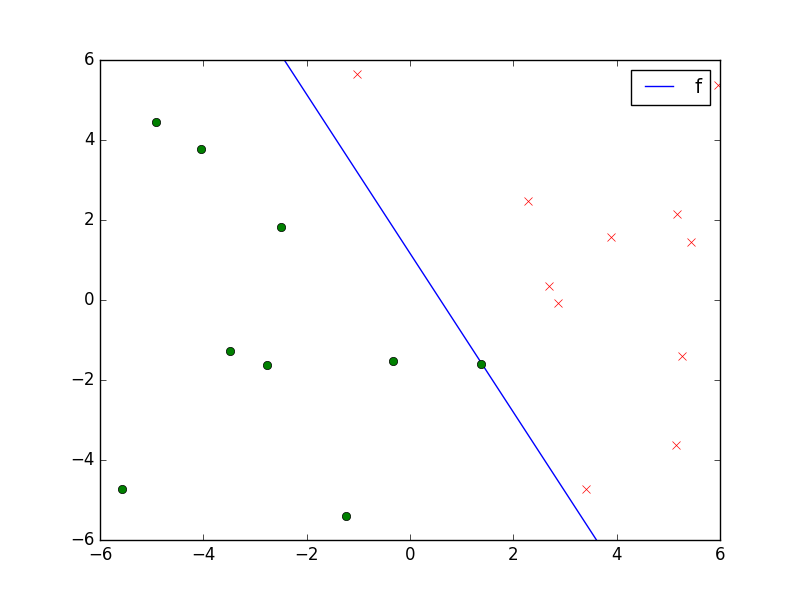
\includegraphics[scale=0.35]{images/3_a.png} 
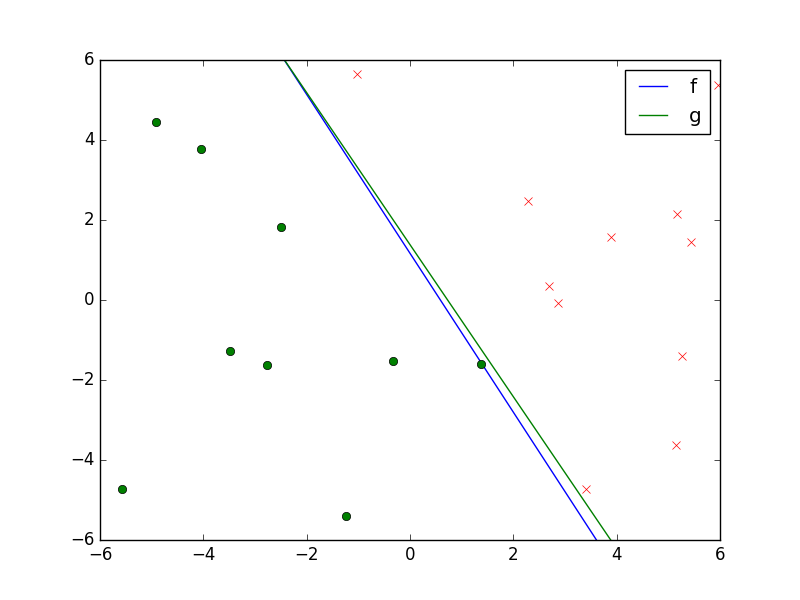
\includegraphics[scale=0.35]{images/3_b.png} 
\end{center}
It took 16 updates of the model and 0.414 ms before converging, for the shown instance. \\
However, I noticed that these numbers can vary a lot so I computed the average time and training steps for 50 instances of the problem (different dataset and different \textit{f}, but same number of data points and dimension of the space), which resulted in an average of 12.2 updates and 0.218 ms.

\item Repeat everything in b) with another randomly generated dataset of size 100, and compare the result to b).
\begin{center}
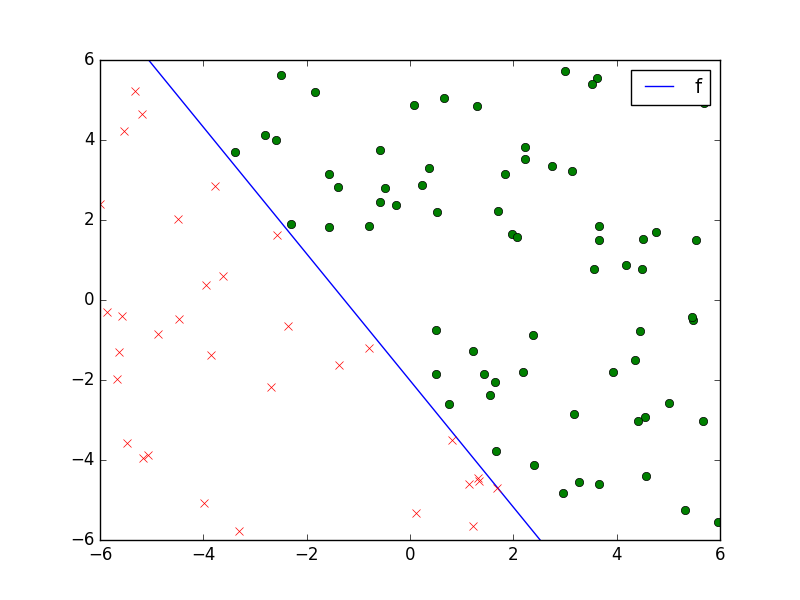
\includegraphics[scale=0.35]{images/4_a.png} 
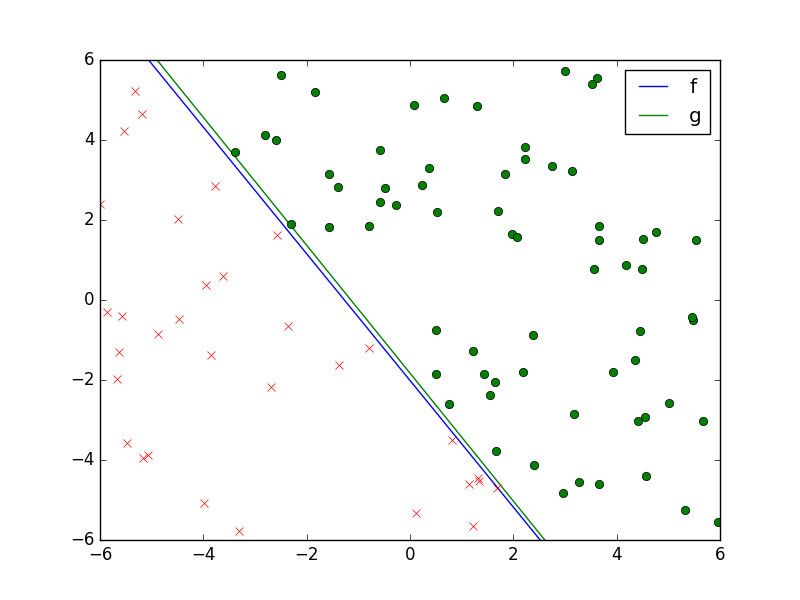
\includegraphics[scale=0.35]{images/4_b.png} 
\end{center}
It took 78 updates of the model and 4.221 ms before converging.\\
Averaging for 50 instances of the problem, it resulted on 87.48 update steps and 2.841 ms of training time.

\item Repeat everything in b) with another randomly generated dataset of size 1000, and compare the result to b).
\begin{center}
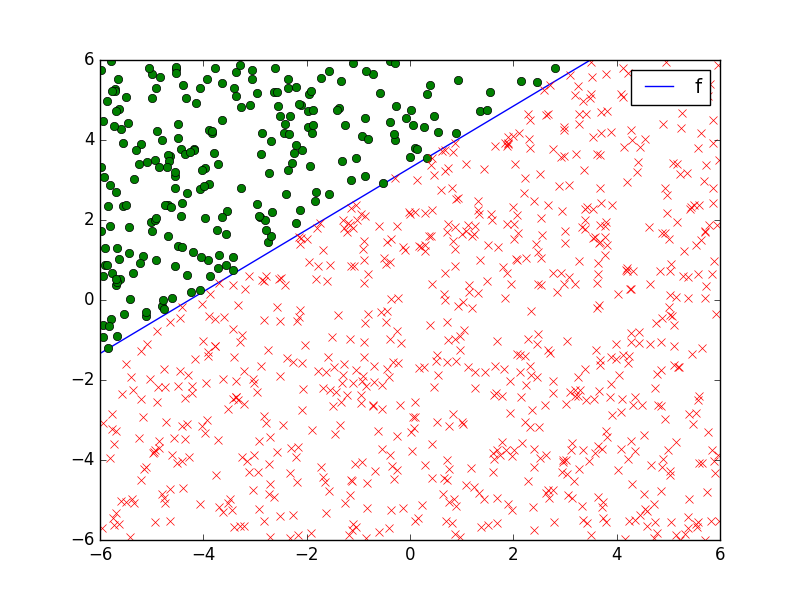
\includegraphics[scale=0.35]{images/5_a.png} 
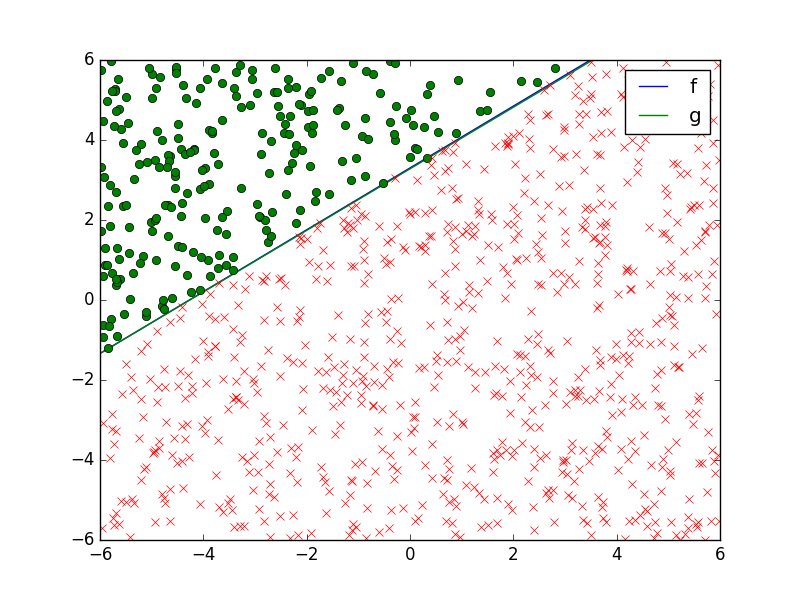
\includegraphics[scale=0.35]{images/5_b.png} 
\end{center}
It took 2176 updates of the model and 195.669 ms before converging.\\
Averaging for 50 instances of the problem, it resulted on 452.7 update steps and 50.815 ms of training time.

\item Modify the experiment such that x\textsubscript{n}$\in$R\textsuperscript{10} instead of R\textsuperscript{2} . Run the algorithm on a randomly generated dataset of size 1000. How many updates does the algorithm take to converge?

It took 6529 updates of the model and 979.125 ms before converging.\\
Averaging for 50 instances of the problem, it resulted on 5908.7 update steps and 737.511 ms of training time.

\item Summarize your conclusions regarding the accuracy and running time of the algorithm as a function of N (the number of data points) and d (the number of dimensions).

\centering
\resizebox{\textwidth}{!}{%
\begin{tabular}{lcccc}
\hline
\multicolumn{1}{c}{} & \multicolumn{1}{l}{N = 20; d = 2} & \multicolumn{1}{l}{N = 100; d = 2} & \multicolumn{1}{l}{N = 1000; d = 2} & \multicolumn{1}{l}{N = 1000; d = 10} \\ \hline
Steps                & 12.2                              & 87.48                              & 452.7                               & 5908.7                               \\ \hline
Time (ms)            & 0.218                             & 2.841                              & 50.815                              & 737.511                              \\ \hline
\end{tabular}%
}



\end{enumerate}


\end{document}